\input{Style/style}
\begin{document}

\begin{titlepage}
%本页为自定义的封面

\newcommand{\paperTitle}{The Road to Trust: Building Enclaves within Confidential VMs }\newcommand{\paperID}{32}
% 定义一个填写信息的命令：宽度7cm，居中
\newcommand{\myinfo}[1]{\underline{\makebox[8cm][c]{\Large #1}}}
% 定义日期填写的命令：宽度较小
\newcommand{\mydate}[1]{\underline{\makebox[1.5cm][c]{\Large #1}}}
~

~

~

~

~



~

~

~

\center{\Huge{华~~中~~科~~技~~大~~学}}\\
\center{\Huge{研究生课程考试答题本}}\\
~

~

~

~
~

~

	\begin{table}[H]
    \centering
    % 增加行高，避免下划线和下一行文字粘连
    \renewcommand{\arraystretch}{2}
    \begin{tabular}{rl}
        {\Large 考生姓名：} & \myinfo{叶一璇} \\
        {\Large 考生学号：} & \myinfo{M202572310} \\
        {\Large 系、年级：} & \myinfo{网络空间安全25级} \\
        {\Large 类~~~~~~~~别：} & \myinfo{硕士} \\ % 使用 ~ 调整"类别"二字的间距
        {\Large 考试科目：} & \myinfo{计算系统安全} \\
        {\Large 考试日期：} & \myinfo{2025年11月26日} \\
    \end{tabular}
\end{table}

\newpage


~



\center{\Huge{评~~~~~~~~分}}\\


~

	\begin{table}[H]
		\centering
        \renewcommand\arraystretch{5}
		  \begin{tabular}{|c|c|c|c|}
            \hline
			{\LARGE ~~~题~~~~~~号~~~}& {\LARGE ~~~得~~~~~~分~~~}& {\LARGE ~~~题~~~~~~号~~~}&{\LARGE ~~~得~~~~~~分~~~}\\ \hline
            \Huge{~ ~}&\Huge{~}&\Huge{~}&\Huge{~}\\ \hline
            \Huge{~ ~}&\Huge{~}&\Huge{~}&\Huge{~}\\ \hline
            \Huge{~ ~}&\Huge{~}&\Huge{~}&\Huge{~}\\ \hline
            \Huge{~ ~}&\Huge{~}&\Huge{~}&\Huge{~}\\ \hline
            \Huge{~ ~}&\Huge{~}&\Huge{~}&\Huge{~}\\ \hline
			
			  \end{tabular}\\
	\end{table}

~

~

	\begin{table}[H]
		\centering
        \renewcommand\arraystretch{5}
		  \begin{tabular}{|l|l|}
            \hline
			{\LARGE 总分：~~~~~~~~~~~~~~~~~~~~~~~~~~~~~}& {\LARGE 评卷人：~~~~~~~~~~~~~~~~~~~~~~~~~~~}\\ \hline
			
			  \end{tabular}\\
	\end{table}

注：1、无评卷人签名试卷无效。~~~~~~~~~~~~~~~~~~~~~~~~~~~~~~~~~~~~~~~~~~~~~~~~~~~~~~~~~~~~~~~~~~~~~~~~~~~~~~~~~~~~~~~~~~~

2、必须用钢笔或圆珠笔阅卷，使用红色。用铅笔阅卷无效。~~~~~~~~~~~~~~~~~~~~~~~~~~~~~


\newpage

        \title{2024年度计算系统安全论文阅读报告   } 
	% \author{作者}
	
    
	\center
	\quad\\
	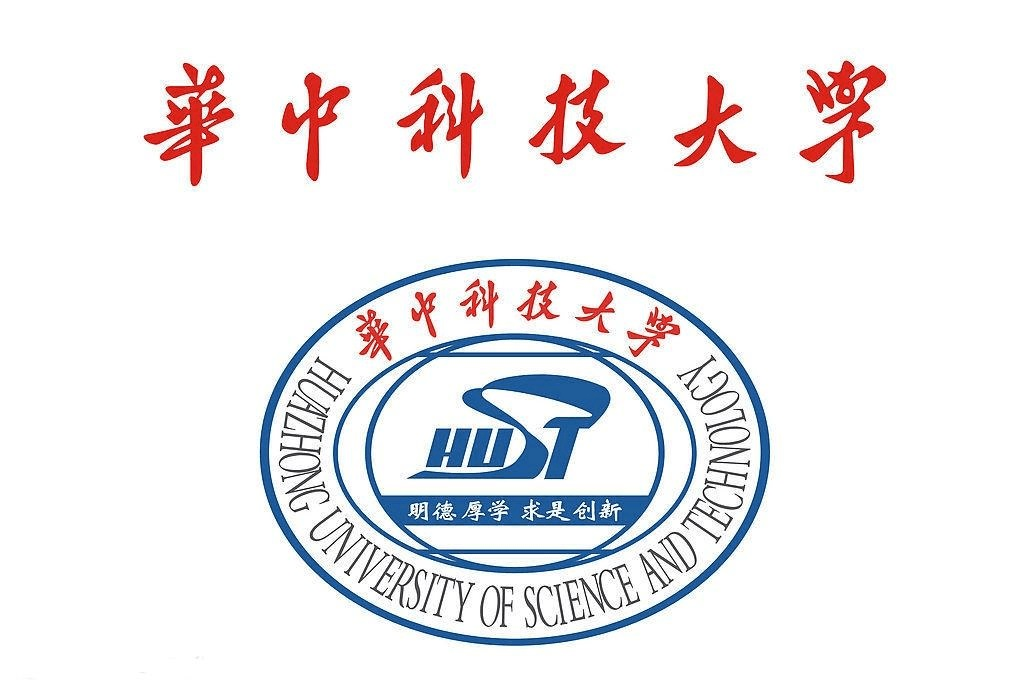
\includegraphics[width=10cm]{Content/logo.jpg}\\
% 	{\Large 题目1}\\[0.5cm]
% 	{\Large 题目2}\\[1.5cm] 
	\quad\\[1cm]
	\makeatletter
	{\linespread{4}\Huge\bfseries\@title}\\[2cm]
	\begin{table}[H]
		\centering
		  \begin{tabular}{rl}
			{\Large 论文题目：}&{\small \paperTitle }\\[0.5cm]
			{\Large 论文编号：}&{\paperID }\\
			  \end{tabular}\\
	\end{table}
	\makeatother
	\quad\\[1cm]
	
	\vfill 
\end{titlepage}%这个是封面，不需要刻意注释掉
\maketitle

\section{论文拟解决的问题}

在当前的云计算环境中，机密计算通过机密虚拟机（CVMs，如AMD SEV-SNP、Intel TDX）保护租户的工作负载免受云服务提供商及恶意宿主机的攻击。然而，现有的CVM模型通常要求用户信任整个虚拟机镜像，这其中包含庞大且复杂的客户机操作系统（Guest OS）。

论文指出的核心问题在于：如何在一个可能被攻陷或不可信的Guest OS中，确保应用程序代码的完整性和安全性？虽然Intel SGX提供了应用层面的Enclave隔离，但其在特定硬件上有局限性；而现有的在AMD SEV上虚拟化SGX的方案（如vSGX）采用了双虚拟机（Two-VM）架构，导致了跨虚拟机边界的控制流传输开销巨大，性能瓶颈严重（例如vSGX的上下文切换比原生SGX慢约160倍）。因此，如何在CVM内部高效地构建受信任的执行环境（TEE），同时保持与现有SGX生态的兼容性，是本论文致力于解决的关键挑战。


\section{论文提出的核心方法}
为了解决上述问题，论文提出了一种名为NestedSGX的框架。该框架利用了AMD SEV-SNP硬件提供的虚拟机特权级（Virtual Machine Privilege Level,VMPL）功能，在单个机密虚拟机内部实现了硬件级的Enclave隔离。

其核心方法包括以下几个方面：

1.利用VMPL实现特权分离：如图1所示，NestedSGX将CVM的执行环境划分为不同的特权级。安全监视器（Security Monitor）和Enclave运行在最高的特权级（如VMPL0），分别处于内核模式和用户模式；而不可信的Guest OS和普通应用程序（App）则运行在较低的特权级（如VMPL1）。这种设计利用硬件强制的内存隔离，确保Guest OS无法访问VMPL0的内存空间。
\begin{figure}[H]
	\center
	\includegraphics*[width=14cm]{Figure/1.jpg}
	\centering
	\caption{嵌套SGX概述}\label{tu1}
\end{figure}

2.SGX兼容性仿真：为了保护现有应用并降低迁移成本，NestedSGX旨在实现与Intel SGX的二进制兼容性,虽然完全二进制兼容非非本文目标，但实现了源代码级的高度兼容。安全监视器充当了受信任的仿真层，负责模拟SGX的叶函数，管理Enclave的生命周期。

3.内存隔离机制：如图2所示，客户机的物理地址空间被划分为三部分：安全监视器专用内存、Enclave专用内存（EPC）和普通内存。通过RMP（Reverse Map Table）检查，硬件保证了低特权级的组件无法访问高特权级的内存区域。

\begin{figure}[H]
	\center
	\includegraphics*[width=12cm]{Figure/2.jpg}
	\centering
	\caption{访客物理地址空间}\label{tu2}
\end{figure}

4.嵌套证明：论文设计了一套信任链机制。安全监视器作为度量信任根（CRTM），负责度量Enclave。最终的证明报告由AMD SEV-SNP的硬件报告和由安全监视器签名的Enclave报告共同组成。

\section{论文贡献总结}
本论文的主要贡献可以归纳为以下三点：

1.创新的架构设计：提出了NestedSGX设计，这是首个利用AMD SEV-SNP的VMPL特性在CVM内部实现应用级Enclave的方案。它采用纵深防御（Defense-in-depth）策略，在不信任Guest OS的前提下为应用提供保护，且避免了vSGX那种多虚拟机架构带来的巨大开销。

2.广泛的兼容性支持：实现了对Intel SGX的高度兼容。作者不仅移植了Intel SGX SDK和Rust SGX SDK，还成功移植了Occlum库操作系统。这使得现有的SGX工具链和应用程序可以无缝集成到NestedSGX中，极大降低了开发者的使用门槛。

3.系统实现与评估：在商用AMD硬件上实现了该系统，并进行了全面的性能评估。结果表明，NestedSGX的开销与原生Intel SGX相当，远优于之前的虚拟化方案（vSGX），证明了该方案的高效性和可行性。

\section{论文实验设计总结与分析}
论文在配备AMD EPYC 7543处理器的服务器上进行了实验，并对比了原生Intel SGX（硬件）、模拟模式（Sim mode）以及之前的相关工作vSGX。

微基准测试：实验显示，NestedSGX在模拟SGX叶指令（如ECREATE,EADD）时，由于只需进行VMPL切换而无需跨VM通信，其速度比vSGX快了数个数量级（如表1所示）。上下文切换的开销大约在32,000到34,000个周期左右，虽然是原生Intel SGX的1.9到2.1倍，但比vSGX快了近两个数量级（vSGX需1.5ms，而NestedSGX仅需12us）。

\begin{table}[htbp]
    \centering
	% \caption{这里写你的表名}
    \caption{vSGX与NestedSGX的指令执行时间对比} \label{t1} 
    \begin{tabular}{clcc} % 4列：居中, 左对齐, 居中, 居中
        \toprule
        & & \textbf{vSGX} & \textbf{NestedSGX} \\
        \midrule
        \multirow{10}{*}{ENCLS} 
        & ECREATE     & 3,719 us & 8.4 us \\
        & EADD        & 1,421 us & 8.0 us \\
        & EEXTEND     & 987 us   & 33 us  \\
        & EINIT       & 811 us   & 46 us  \\
        & EREMOVE     & 1,014 us & 7.8 us \\
        & EAUG        & 990 us   & 7.9 us \\
        & EBLOCK      & 841 us   & 9.2 us \\
        & ELDB/ELDU   & 1,958 us & 9.3 us \\
        & EMODPR      & 1,071 us & 9.9 us \\
        & EWB         & 1,819 us & 7.9 us \\
        \midrule
        \multirow{2}{*}{ENCLU} 
        & EGETKEY     & 5.0 us   & 17 us \\
        & EREPORT     & 19 us    & 30 us \\
        \bottomrule
    \end{tabular}
\end{table}


真实应用测试：在Nbench、Lmbench和WolfSSL测试中，如图3所示，NestedSGX的平均开销非常低（低于2\%）。例如，WolfSSL的平均开销仅为0.78\%。使用FIO和Redis（运行在Occlum上）进行测试。如图4所示，Redis在高吞吐量下的额外开销约为15.68\%。这主要是由于I/O操作需要频繁的系统调用和模式切换，但通过HotCalls优化，性能已在可接受范围内。在Hashjoin和SQLite测试中，开销同样微乎其微（SQLite开销约0.77\%）。

\begin{figure}[H]
	\center
	\includegraphics*[width=16cm]{Figure/3.jpg}
	\centering
	\caption{微基准测试}\label{tu3}
\end{figure}

\begin{figure}[H]
	\center
	\includegraphics*[width=16cm]{Figure/4.jpg}
	\centering
	\caption{真实应用测试}\label{tu4}
\end{figure}

分析：实验设计涵盖了从底层指令到高层复杂应用的全方位测试。结果有力地证明了VMPL架构在性能上的优势，尤其是在避免了跨VM通信后，不仅解决了vSGX的性能瓶颈，还在计算密集型任务上逼近了原生硬件的性能表现。


\section{论文阅读心得}
首先，信任粒度的细化是云安全发展的必然趋势。传统的机密虚拟机（CVM）虽然隔离了云厂商，但将巨大的Guest OS纳入信任计算基（TCB）本身就是一种风险。NestedSGX将信任边界从“整个虚拟机”收缩回“Enclave”，这种回归Intel SGX原始理念但又构建在新型CVM硬件之上的做法，非常符合最小特权原则。

其次，软硬件协同设计的重要性再次凸显。论文巧妙地利用了AMD SEV-SNP的VMPL特性。VMPL本意可能更多是为了支持vTPM或热迁移等管理功能，但作者将其用于构建用户态的隔离环境，这是一种非常精彩的“借力打力”。相较于vSGX强行用软件模拟硬件行为导致的性能损耗，NestedSGX是顺应硬件特性的架构创新。

最后，兼容性是技术落地的关键。作者花费大量精力移植SGX SDK和Occlum，使得该方案不仅停留在理论模型上，而是真正可以直接运行现有的SGX应用（如Redis,SQLite）。这种对生态兼容性的重视，使得NestedSGX具有极高的实用价值和工业界应用潜力。

尽管在I/O密集型场景下仍有一定开销（约15\%），且目前设计主要针对AMD平台，但其提出的利用VM内部特权级隔离来构建Enclave的思路，对于未来Intel TDX或ARM CCA的生态演进都具有重要的借鉴意义。

\nocite{*}
\printbibliography
\end{document}